% !TEX root = ../../main.tex


\begin{figure}[p]
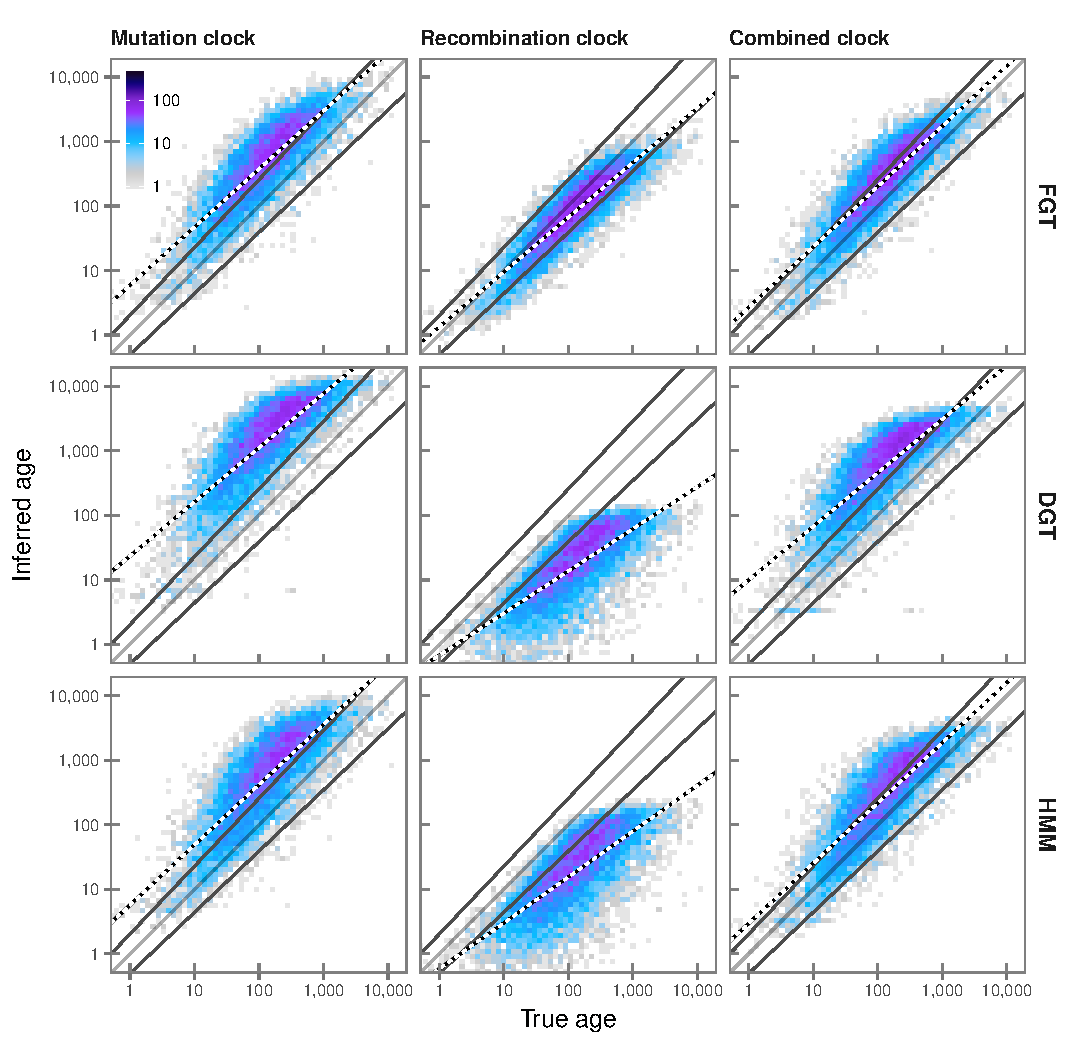
\includegraphics[width=\textwidth]{./img/ch5/vanilla_scat}
\Caption{Distribution of true and inferred age using different IBD detection methods}
{The \n{3} IBD detection methods implemented in \texttt{rvage} were compared, \ie \gls{fgt}, \gls{dgt}, and \gls{hmm} (indicated at the \emph{right} of each row), under each clock model (indicated at the \emph{top} of each column).
Analyses were compared on the same set of \n{9434} target sites that were drawn from available \fk{[2,20]} variants in the simulated dataset of \n{2000} haplotypes (allele frequency ${\leq 1\%}$).
Each panel shows the density of true age ($t_m$) and inferred age (numbers indicated by the colour-gradient).
Lines \emph{below} and \emph{above} the dividing line are regression trend lines of the corresponding true coalescent times around each mutation event, $t_c$ and $t_d$, respectively.
The regression trend line of inferred age ($\hat{t}$) is indicated by the \emph{black-white} line, using the posterior mode of the composite likelihood estimation as the inferred age value.}
{fig:vanilla_scat}
\end{figure}
